\PassOptionsToPackage{table}{xcolor}
\documentclass{book}\usepackage[]{graphicx}\usepackage[]{color}
% maxwidth is the original width if it is less than linewidth
% otherwise use linewidth (to make sure the graphics do not exceed the margin)
\makeatletter
\def\maxwidth{ %
  \ifdim\Gin@nat@width>\linewidth
    \linewidth
  \else
    \Gin@nat@width
  \fi
}
\makeatother

\definecolor{fgcolor}{rgb}{0.345, 0.345, 0.345}
\newcommand{\hlnum}[1]{\textcolor[rgb]{0.686,0.059,0.569}{#1}}%
\newcommand{\hlstr}[1]{\textcolor[rgb]{0.192,0.494,0.8}{#1}}%
\newcommand{\hlcom}[1]{\textcolor[rgb]{0.678,0.584,0.686}{\textit{#1}}}%
\newcommand{\hlopt}[1]{\textcolor[rgb]{0,0,0}{#1}}%
\newcommand{\hlstd}[1]{\textcolor[rgb]{0.345,0.345,0.345}{#1}}%
\newcommand{\hlkwa}[1]{\textcolor[rgb]{0.161,0.373,0.58}{\textbf{#1}}}%
\newcommand{\hlkwb}[1]{\textcolor[rgb]{0.69,0.353,0.396}{#1}}%
\newcommand{\hlkwc}[1]{\textcolor[rgb]{0.333,0.667,0.333}{#1}}%
\newcommand{\hlkwd}[1]{\textcolor[rgb]{0.737,0.353,0.396}{\textbf{#1}}}%
\let\hlipl\hlkwb

\usepackage{framed}
\makeatletter
\newenvironment{kframe}{%
 \def\at@end@of@kframe{}%
 \ifinner\ifhmode%
  \def\at@end@of@kframe{\end{minipage}}%
  \begin{minipage}{\columnwidth}%
 \fi\fi%
 \def\FrameCommand##1{\hskip\@totalleftmargin \hskip-\fboxsep
 \colorbox{shadecolor}{##1}\hskip-\fboxsep
     % There is no \\@totalrightmargin, so:
     \hskip-\linewidth \hskip-\@totalleftmargin \hskip\columnwidth}%
 \MakeFramed {\advance\hsize-\width
   \@totalleftmargin\z@ \linewidth\hsize
   \@setminipage}}%
 {\par\unskip\endMakeFramed%
 \at@end@of@kframe}
\makeatother

\definecolor{shadecolor}{rgb}{.97, .97, .97}
\definecolor{messagecolor}{rgb}{0, 0, 0}
\definecolor{warningcolor}{rgb}{1, 0, 1}
\definecolor{errorcolor}{rgb}{1, 0, 0}
\newenvironment{knitrout}{}{} % an empty environment to be redefined in TeX

\usepackage{alltt}
\usepackage[a4paper, top=3cm, bottom=3cm, left=2cm, right=2cm]{geometry}
\usepackage[utf8]{inputenc}
\usepackage{setspace}
\usepackage{tocloft}
\usepackage{makeidx}
\usepackage{relsize,setspace}
\usepackage{rotating}
\usepackage{lscape}
\usepackage{hyperref}
\usepackage{indentfirst}
%------- for kableExtra package in R, start
\usepackage{booktabs}
\usepackage{longtable}
\usepackage{array}
\usepackage{multirow}
\usepackage[table]{xcolor}
\usepackage{wrapfig}
\usepackage{float}
\usepackage{colortbl}
\usepackage{pdflscape}
\usepackage{tabu}
\usepackage{threeparttable}
\usepackage[normalem]{ulem}
%------- for kableExtra package in R, end

\hypersetup{
    colorlinks,
    citecolor=black,
    filecolor=black,
    linkcolor=black,
    urlcolor=black
}

\makeindex
\IfFileExists{upquote.sty}{\usepackage{upquote}}{}
\begin{document}

\newcommand{\HRule}{\rule{\linewidth}{0.5mm}}

%------- title page
\begin{titlepage}
\begin{center}

\begin{minipage}{0.4\textwidth}
\begin{flushleft} \large

\includegraphics[width=0.4\textwidth]{./img/Rlogo}~\\[1cm]
\end{flushleft}
\end{minipage}
\begin{minipage}{0.4\textwidth}
\begin{flushright} \large

\includegraphics[width=0.3\textwidth]{./img/detective_2}~\\[1cm]
\end{flushright}
\end{minipage}\\[4.5cm]

\textsc{\Large report series with dlookr}\\[1.0cm]

% Title
\HRule \\[0.4cm]
{ \huge \bfseries Exploratory Data Analysis Report \\[0.4cm] }

\HRule \\[4.5cm]

% Author and package version
\begin{minipage}{0.4\textwidth}
\begin{flushleft} \large
\emph{Author:}\\
dlookr package
\end{flushleft}
\end{minipage}
\begin{minipage}{0.4\textwidth}
\begin{flushright} \large
\emph{Version:} \\
0.3.12
\end{flushright}
\end{minipage}

\vfill

% Bottom of the page
{\large \today}

\end{center}
\end{titlepage}

% Last pages for ToC
%-------------------------------------------------------------------------------
\newpage
% Include dots between chapter name and page number
\renewcommand{\cftchapdotsep}{\cftdotsep}
% Last pages for ToC
%-------------------------------------------------------------------------------
% Include the ToC
\tableofcontents


% !Rnw root = EDA_Report.Rnw





\chapter{Introduction}
The EDA Report provides exploratory data analysis information on objects that inherit data.frame and data.frame.

\section{Information of Dataset}
The dataset that generated the EDA Report is an 'data.frame' object. It consists of 218 observations and 12 variables.

\section{Information of Variables}
\begin{table}[!h]

\caption{\label{tab:info_variables}Information of Variables}
\centering
\begin{tabular}[t]{llrrrr}
\toprule
variables & types & missing\_count & missing\_percent & unique\_count & unique\_rate\\
\midrule
\cellcolor{gray!6}{countrycode} & \cellcolor{gray!6}{character} & \cellcolor{gray!6}{0} & \cellcolor{gray!6}{0.000000} & \cellcolor{gray!6}{218} & \cellcolor{gray!6}{1.0000000}\\
logGDPpc2000 & numeric & 24 & 11.009174 & 195 & 0.8944954\\
\cellcolor{gray!6}{logGDPpc2015} & \cellcolor{gray!6}{numeric} & \cellcolor{gray!6}{18} & \cellcolor{gray!6}{8.256881} & \cellcolor{gray!6}{201} & \cellcolor{gray!6}{0.9220183}\\
growthGDPpc & numeric & 26 & 11.926606 & 193 & 0.8853211\\
\cellcolor{gray!6}{imalaria2000} & \cellcolor{gray!6}{numeric} & \cellcolor{gray!6}{119} & \cellcolor{gray!6}{54.587156} & \cellcolor{gray!6}{100} & \cellcolor{gray!6}{0.4587156}\\
\addlinespace
imalaria2015 & numeric & 119 & 54.587156 & 86 & 0.3944954\\
\cellcolor{gray!6}{change\_malar} & \cellcolor{gray!6}{numeric} & \cellcolor{gray!6}{119} & \cellcolor{gray!6}{54.587156} & \cellcolor{gray!6}{98} & \cellcolor{gray!6}{0.4495413}\\
educ\_sec & numeric & 119 & 54.587156 & 100 & 0.4587156\\
\cellcolor{gray!6}{life2000} & \cellcolor{gray!6}{numeric} & \cellcolor{gray!6}{17} & \cellcolor{gray!6}{7.798165} & \cellcolor{gray!6}{201} & \cellcolor{gray!6}{0.9220183}\\
trade2000 & numeric & 40 & 18.348624 & 179 & 0.8211009\\
\addlinespace
\cellcolor{gray!6}{gov2000} & \cellcolor{gray!6}{numeric} & \cellcolor{gray!6}{25} & \cellcolor{gray!6}{11.467890} & \cellcolor{gray!6}{190} & \cellcolor{gray!6}{0.8715596}\\
invest\_growth & numeric & 91 & 41.743119 & 128 & 0.5871560\\
\bottomrule
\end{tabular}
\end{table}

The target variable of the data is 'NULL', and the data type of the variable is NULL(You did not specify a target variable).

\section{About EDA Report}
EDA reports provide information and visualization results that support the EDA process. In particular, it provides a variety of information to understand the relationship between the target variable and the rest of the variables of interest.

\chapter{Univariate Analysis}
\section{Descriptive Statistics}

\begin{spacing}{0.7}
\begin{center}\textbf{ edaData \\ 12 Variables~~~~~ 218 ~Observations}\end{center}
\smallskip\hrule\smallskip{\small
\vbox{\noindent\textbf{countrycode : Country Code}{\smaller~~Format:\%9s}

{\smaller
\begin{tabular}{ rrr }
n&missing&distinct \\
218&0&218 \end{tabular}
\begin{verbatim}

lowest : ABW AFG AGO ALB AND, highest: XKX YEM ZAF ZMB ZWE
\end{verbatim}
}
\smallskip\hrule\smallskip
}
\vbox{\noindent\textbf{logGDPpc2000 : Log GDPpc 2000}{\smaller~~Format:\%9.0g}\setlength{\unitlength}{0.001in}\hfill\begin{picture}(1.5,.1)(1500,0)\linethickness{0.6pt}
\put(0,0){\line(0,1){14}}
\put(34,0){\line(0,1){14}}
\put(79,0){\line(0,1){29}}
\put(91,0){\line(0,1){14}}
\put(113,0){\line(0,1){29}}
\put(125,0){\line(0,1){14}}
\put(147,0){\line(0,1){14}}
\put(170,0){\line(0,1){71}}
\put(181,0){\line(0,1){14}}
\put(193,0){\line(0,1){14}}
\put(204,0){\line(0,1){14}}
\put(215,0){\line(0,1){43}}
\put(227,0){\line(0,1){29}}
\put(249,0){\line(0,1){29}}
\put(272,0){\line(0,1){29}}
\put(283,0){\line(0,1){14}}
\put(306,0){\line(0,1){29}}
\put(317,0){\line(0,1){71}}
\put(329,0){\line(0,1){14}}
\put(351,0){\line(0,1){29}}
\put(363,0){\line(0,1){29}}
\put(374,0){\line(0,1){14}}
\put(385,0){\line(0,1){14}}
\put(397,0){\line(0,1){57}}
\put(419,0){\line(0,1){43}}
\put(431,0){\line(0,1){29}}
\put(442,0){\line(0,1){29}}
\put(453,0){\line(0,1){14}}
\put(476,0){\line(0,1){100}}
\put(487,0){\line(0,1){14}}
\put(499,0){\line(0,1){43}}
\put(510,0){\line(0,1){14}}
\put(521,0){\line(0,1){29}}
\put(533,0){\line(0,1){14}}
\put(544,0){\line(0,1){57}}
\put(566,0){\line(0,1){43}}
\put(578,0){\line(0,1){14}}
\put(589,0){\line(0,1){43}}
\put(600,0){\line(0,1){57}}
\put(612,0){\line(0,1){29}}
\put(623,0){\line(0,1){29}}
\put(634,0){\line(0,1){43}}
\put(646,0){\line(0,1){57}}
\put(657,0){\line(0,1){43}}
\put(668,0){\line(0,1){14}}
\put(680,0){\line(0,1){43}}
\put(691,0){\line(0,1){14}}
\put(702,0){\line(0,1){14}}
\put(714,0){\line(0,1){29}}
\put(725,0){\line(0,1){57}}
\put(736,0){\line(0,1){14}}
\put(748,0){\line(0,1){29}}
\put(759,0){\line(0,1){71}}
\put(770,0){\line(0,1){14}}
\put(782,0){\line(0,1){29}}
\put(793,0){\line(0,1){14}}
\put(804,0){\line(0,1){43}}
\put(816,0){\line(0,1){14}}
\put(838,0){\line(0,1){29}}
\put(850,0){\line(0,1){14}}
\put(861,0){\line(0,1){43}}
\put(872,0){\line(0,1){43}}
\put(884,0){\line(0,1){43}}
\put(895,0){\line(0,1){57}}
\put(929,0){\line(0,1){14}}
\put(952,0){\line(0,1){14}}
\put(963,0){\line(0,1){14}}
\put(974,0){\line(0,1){29}}
\put(986,0){\line(0,1){14}}
\put(1020,0){\line(0,1){29}}
\put(1031,0){\line(0,1){29}}
\put(1065,0){\line(0,1){29}}
\put(1076,0){\line(0,1){43}}
\put(1088,0){\line(0,1){14}}
\put(1110,0){\line(0,1){14}}
\put(1122,0){\line(0,1){43}}
\put(1133,0){\line(0,1){14}}
\put(1144,0){\line(0,1){14}}
\put(1156,0){\line(0,1){14}}
\put(1167,0){\line(0,1){14}}
\put(1178,0){\line(0,1){57}}
\put(1190,0){\line(0,1){43}}
\put(1201,0){\line(0,1){57}}
\put(1212,0){\line(0,1){29}}
\put(1224,0){\line(0,1){57}}
\put(1235,0){\line(0,1){29}}
\put(1280,0){\line(0,1){14}}
\put(1292,0){\line(0,1){14}}
\put(1303,0){\line(0,1){14}}
\put(1314,0){\line(0,1){14}}
\put(1326,0){\line(0,1){14}}
\put(1360,0){\line(0,1){29}}
\put(1382,0){\line(0,1){14}}
\put(1394,0){\line(0,1){14}}
\put(1484,0){\line(0,1){14}}
\end{picture}

{\smaller[2]
\begin{tabular}{ rrrrrrrrrrrrr }
n&missing&distinct&Info&Mean&Gmd&.05&.10&.25&.50&.75&.90&.95 \\
194&24&194&1&8.39&1.8& 6.035& 6.285& 7.195& 8.222& 9.618&10.601&10.810 \end{tabular}
\begin{verbatim}

lowest :  5.285396  5.434622  5.667314  5.669834  5.711302
highest: 11.289637 11.310238 11.410585 11.445320 11.840078
\end{verbatim}
}
\smallskip\hrule\smallskip
}
\vbox{\noindent\textbf{logGDPpc2015 : Log GDPpc 2015}{\smaller~~Format:\%9.0g}\setlength{\unitlength}{0.001in}\hfill\begin{picture}(1.5,.1)(1500,0)\linethickness{0.6pt}
\put(0,0){\line(0,1){17}}
\put(89,0){\line(0,1){17}}
\put(111,0){\line(0,1){17}}
\put(122,0){\line(0,1){17}}
\put(144,0){\line(0,1){17}}
\put(155,0){\line(0,1){17}}
\put(166,0){\line(0,1){17}}
\put(177,0){\line(0,1){17}}
\put(199,0){\line(0,1){67}}
\put(222,0){\line(0,1){33}}
\put(244,0){\line(0,1){17}}
\put(255,0){\line(0,1){100}}
\put(266,0){\line(0,1){17}}
\put(277,0){\line(0,1){17}}
\put(288,0){\line(0,1){17}}
\put(299,0){\line(0,1){17}}
\put(310,0){\line(0,1){33}}
\put(321,0){\line(0,1){17}}
\put(332,0){\line(0,1){33}}
\put(343,0){\line(0,1){33}}
\put(366,0){\line(0,1){33}}
\put(388,0){\line(0,1){50}}
\put(399,0){\line(0,1){50}}
\put(410,0){\line(0,1){33}}
\put(421,0){\line(0,1){17}}
\put(432,0){\line(0,1){50}}
\put(443,0){\line(0,1){33}}
\put(454,0){\line(0,1){17}}
\put(465,0){\line(0,1){17}}
\put(488,0){\line(0,1){33}}
\put(510,0){\line(0,1){33}}
\put(521,0){\line(0,1){17}}
\put(532,0){\line(0,1){33}}
\put(543,0){\line(0,1){50}}
\put(554,0){\line(0,1){67}}
\put(565,0){\line(0,1){17}}
\put(576,0){\line(0,1){33}}
\put(587,0){\line(0,1){50}}
\put(598,0){\line(0,1){33}}
\put(609,0){\line(0,1){50}}
\put(620,0){\line(0,1){100}}
\put(643,0){\line(0,1){33}}
\put(654,0){\line(0,1){50}}
\put(665,0){\line(0,1){50}}
\put(676,0){\line(0,1){17}}
\put(687,0){\line(0,1){17}}
\put(698,0){\line(0,1){50}}
\put(709,0){\line(0,1){17}}
\put(720,0){\line(0,1){67}}
\put(731,0){\line(0,1){50}}
\put(742,0){\line(0,1){100}}
\put(753,0){\line(0,1){17}}
\put(765,0){\line(0,1){33}}
\put(776,0){\line(0,1){67}}
\put(787,0){\line(0,1){33}}
\put(798,0){\line(0,1){17}}
\put(809,0){\line(0,1){17}}
\put(820,0){\line(0,1){50}}
\put(831,0){\line(0,1){50}}
\put(842,0){\line(0,1){33}}
\put(853,0){\line(0,1){33}}
\put(864,0){\line(0,1){33}}
\put(886,0){\line(0,1){17}}
\put(897,0){\line(0,1){50}}
\put(909,0){\line(0,1){83}}
\put(920,0){\line(0,1){67}}
\put(931,0){\line(0,1){33}}
\put(942,0){\line(0,1){33}}
\put(953,0){\line(0,1){17}}
\put(964,0){\line(0,1){17}}
\put(975,0){\line(0,1){17}}
\put(997,0){\line(0,1){33}}
\put(1008,0){\line(0,1){33}}
\put(1019,0){\line(0,1){17}}
\put(1030,0){\line(0,1){50}}
\put(1042,0){\line(0,1){17}}
\put(1053,0){\line(0,1){33}}
\put(1064,0){\line(0,1){17}}
\put(1075,0){\line(0,1){17}}
\put(1086,0){\line(0,1){17}}
\put(1097,0){\line(0,1){50}}
\put(1108,0){\line(0,1){17}}
\put(1119,0){\line(0,1){50}}
\put(1141,0){\line(0,1){17}}
\put(1152,0){\line(0,1){50}}
\put(1163,0){\line(0,1){33}}
\put(1174,0){\line(0,1){83}}
\put(1197,0){\line(0,1){67}}
\put(1208,0){\line(0,1){50}}
\put(1219,0){\line(0,1){17}}
\put(1230,0){\line(0,1){17}}
\put(1252,0){\line(0,1){33}}
\put(1274,0){\line(0,1){17}}
\put(1285,0){\line(0,1){17}}
\put(1296,0){\line(0,1){17}}
\put(1318,0){\line(0,1){17}}
\put(1363,0){\line(0,1){17}}
\put(1485,0){\line(0,1){17}}
\end{picture}

{\smaller[2]
\begin{tabular}{ rrrrrrrrrrrrr }
n&missing&distinct&Info&Mean&Gmd&.05&.10&.25&.50&.75&.90&.95 \\
200&18&200&1&8.719&1.69& 6.353& 6.618& 7.609& 8.745& 9.794&10.732&10.917 \end{tabular}
\begin{verbatim}

lowest :  5.431241  5.847467  5.956626  6.018643  6.089357
highest: 11.245743 11.307289 11.407891 11.586531 12.151471
\end{verbatim}
}
\smallskip\hrule\smallskip
}
\vbox{\noindent\textbf{growthGDPpc : Av. GDPpc growth 2015-2000}{\smaller~~Format:\%9.0g}\setlength{\unitlength}{0.001in}\hfill\begin{picture}(1.5,.1)(1500,0)\linethickness{0.6pt}
\put(0,0){\line(0,1){17}}
\put(24,0){\line(0,1){17}}
\put(122,0){\line(0,1){17}}
\put(159,0){\line(0,1){17}}
\put(208,0){\line(0,1){33}}
\put(233,0){\line(0,1){17}}
\put(245,0){\line(0,1){17}}
\put(257,0){\line(0,1){17}}
\put(269,0){\line(0,1){17}}
\put(282,0){\line(0,1){17}}
\put(294,0){\line(0,1){17}}
\put(306,0){\line(0,1){17}}
\put(318,0){\line(0,1){33}}
\put(331,0){\line(0,1){17}}
\put(343,0){\line(0,1){50}}
\put(355,0){\line(0,1){17}}
\put(367,0){\line(0,1){67}}
\put(379,0){\line(0,1){50}}
\put(392,0){\line(0,1){33}}
\put(404,0){\line(0,1){50}}
\put(416,0){\line(0,1){17}}
\put(428,0){\line(0,1){83}}
\put(441,0){\line(0,1){50}}
\put(453,0){\line(0,1){67}}
\put(465,0){\line(0,1){50}}
\put(477,0){\line(0,1){100}}
\put(490,0){\line(0,1){50}}
\put(502,0){\line(0,1){50}}
\put(514,0){\line(0,1){100}}
\put(526,0){\line(0,1){17}}
\put(539,0){\line(0,1){100}}
\put(551,0){\line(0,1){100}}
\put(563,0){\line(0,1){50}}
\put(575,0){\line(0,1){100}}
\put(588,0){\line(0,1){83}}
\put(600,0){\line(0,1){17}}
\put(612,0){\line(0,1){67}}
\put(624,0){\line(0,1){33}}
\put(637,0){\line(0,1){33}}
\put(649,0){\line(0,1){83}}
\put(661,0){\line(0,1){33}}
\put(673,0){\line(0,1){67}}
\put(686,0){\line(0,1){100}}
\put(698,0){\line(0,1){33}}
\put(722,0){\line(0,1){67}}
\put(735,0){\line(0,1){83}}
\put(747,0){\line(0,1){33}}
\put(759,0){\line(0,1){33}}
\put(771,0){\line(0,1){67}}
\put(783,0){\line(0,1){50}}
\put(796,0){\line(0,1){17}}
\put(808,0){\line(0,1){67}}
\put(820,0){\line(0,1){67}}
\put(832,0){\line(0,1){17}}
\put(845,0){\line(0,1){50}}
\put(857,0){\line(0,1){17}}
\put(869,0){\line(0,1){33}}
\put(881,0){\line(0,1){33}}
\put(894,0){\line(0,1){17}}
\put(906,0){\line(0,1){17}}
\put(918,0){\line(0,1){33}}
\put(930,0){\line(0,1){50}}
\put(943,0){\line(0,1){33}}
\put(955,0){\line(0,1){33}}
\put(979,0){\line(0,1){17}}
\put(1004,0){\line(0,1){33}}
\put(1016,0){\line(0,1){33}}
\put(1028,0){\line(0,1){17}}
\put(1041,0){\line(0,1){33}}
\put(1065,0){\line(0,1){33}}
\put(1077,0){\line(0,1){33}}
\put(1090,0){\line(0,1){33}}
\put(1102,0){\line(0,1){17}}
\put(1126,0){\line(0,1){17}}
\put(1138,0){\line(0,1){17}}
\put(1200,0){\line(0,1){17}}
\put(1212,0){\line(0,1){17}}
\put(1420,0){\line(0,1){17}}
\put(1432,0){\line(0,1){17}}
\put(1481,0){\line(0,1){17}}
\end{picture}

{\smaller
\begin{verbatim}
       n  missing distinct     Info     Mean      Gmd      .05      .10      .25      .50 
     192       26      192        1    2.276    2.355  -0.7001  -0.1279   0.8492   1.9916 
     .75      .90      .95 
  3.5759   5.2073   5.8420 

lowest : -3.013770 -2.788296 -2.009163 -1.677084 -1.348502
highest:  6.849905  6.890720  8.641517  8.664331  9.077437
\end{verbatim}
}
\smallskip\hrule\smallskip
}
\vbox{\noindent\textbf{imalaria2000 : Malaria incidence rate in 2000}{\smaller~~Format:\%9.0g}\setlength{\unitlength}{0.001in}\hfill\begin{picture}(1.5,.1)(1500,0)\linethickness{0.6pt}
\put(0,0){\line(0,1){100}}
\put(4,0){\line(0,1){100}}
\put(7,0){\line(0,1){100}}
\put(11,0){\line(0,1){83}}
\put(15,0){\line(0,1){100}}
\put(19,0){\line(0,1){67}}
\put(22,0){\line(0,1){33}}
\put(26,0){\line(0,1){67}}
\put(41,0){\line(0,1){50}}
\put(44,0){\line(0,1){17}}
\put(56,0){\line(0,1){17}}
\put(67,0){\line(0,1){17}}
\put(74,0){\line(0,1){17}}
\put(82,0){\line(0,1){17}}
\put(89,0){\line(0,1){17}}
\put(93,0){\line(0,1){17}}
\put(108,0){\line(0,1){17}}
\put(115,0){\line(0,1){33}}
\put(122,0){\line(0,1){33}}
\put(130,0){\line(0,1){17}}
\put(171,0){\line(0,1){17}}
\put(185,0){\line(0,1){17}}
\put(193,0){\line(0,1){17}}
\put(204,0){\line(0,1){17}}
\put(230,0){\line(0,1){17}}
\put(234,0){\line(0,1){17}}
\put(245,0){\line(0,1){17}}
\put(300,0){\line(0,1){17}}
\put(341,0){\line(0,1){17}}
\put(400,0){\line(0,1){17}}
\put(408,0){\line(0,1){17}}
\put(411,0){\line(0,1){17}}
\put(426,0){\line(0,1){17}}
\put(493,0){\line(0,1){17}}
\put(508,0){\line(0,1){17}}
\put(526,0){\line(0,1){17}}
\put(541,0){\line(0,1){17}}
\put(549,0){\line(0,1){33}}
\put(586,0){\line(0,1){17}}
\put(608,0){\line(0,1){17}}
\put(619,0){\line(0,1){17}}
\put(638,0){\line(0,1){17}}
\put(682,0){\line(0,1){17}}
\put(697,0){\line(0,1){17}}
\put(701,0){\line(0,1){33}}
\put(734,0){\line(0,1){17}}
\put(738,0){\line(0,1){17}}
\put(753,0){\line(0,1){33}}
\put(775,0){\line(0,1){17}}
\put(786,0){\line(0,1){17}}
\put(801,0){\line(0,1){17}}
\put(819,0){\line(0,1){17}}
\put(838,0){\line(0,1){17}}
\put(849,0){\line(0,1){17}}
\put(860,0){\line(0,1){17}}
\put(923,0){\line(0,1){17}}
\put(953,0){\line(0,1){17}}
\put(1094,0){\line(0,1){17}}
\put(1127,0){\line(0,1){17}}
\put(1157,0){\line(0,1){17}}
\put(1475,0){\line(0,1){17}}
\end{picture}

{\smaller[2]
\begin{tabular}{ rrrrrrrrrrrrr }
n&missing&distinct&Info&Mean&Gmd&.05&.10&.25&.50&.75&.90&.95 \\
99&119&99&1&159.9&201&  0.628&  2.594&  8.105& 57.310&305.990&434.374&500.148 \end{tabular}
\begin{verbatim}

lowest :   0.01   0.30   0.31   0.38   0.61, highest: 514.62 589.59 607.11 623.24 796.38
\end{verbatim}
}
\smallskip\hrule\smallskip
}
\vbox{\noindent\textbf{imalaria2015 : Malaria incidence rate in 2015}{\smaller~~Format:\%9.0g}\setlength{\unitlength}{0.001in}\hfill\begin{picture}(1.5,.1)(1500,0)\linethickness{0.6pt}
\put(0,0){\line(0,1){100}}
\put(3,0){\line(0,1){23}}
\put(7,0){\line(0,1){10}}
\put(10,0){\line(0,1){10}}
\put(14,0){\line(0,1){3}}
\put(17,0){\line(0,1){6}}
\put(24,0){\line(0,1){6}}
\put(34,0){\line(0,1){6}}
\put(38,0){\line(0,1){3}}
\put(45,0){\line(0,1){3}}
\put(48,0){\line(0,1){6}}
\put(55,0){\line(0,1){3}}
\put(69,0){\line(0,1){3}}
\put(79,0){\line(0,1){6}}
\put(127,0){\line(0,1){3}}
\put(130,0){\line(0,1){3}}
\put(168,0){\line(0,1){3}}
\put(182,0){\line(0,1){3}}
\put(206,0){\line(0,1){6}}
\put(237,0){\line(0,1){3}}
\put(250,0){\line(0,1){3}}
\put(271,0){\line(0,1){3}}
\put(298,0){\line(0,1){3}}
\put(388,0){\line(0,1){3}}
\put(401,0){\line(0,1){3}}
\put(463,0){\line(0,1){3}}
\put(504,0){\line(0,1){3}}
\put(521,0){\line(0,1){3}}
\put(528,0){\line(0,1){3}}
\put(593,0){\line(0,1){3}}
\put(658,0){\line(0,1){3}}
\put(665,0){\line(0,1){3}}
\put(689,0){\line(0,1){3}}
\put(700,0){\line(0,1){3}}
\put(713,0){\line(0,1){3}}
\put(717,0){\line(0,1){6}}
\put(799,0){\line(0,1){3}}
\put(933,0){\line(0,1){3}}
\put(998,0){\line(0,1){3}}
\put(1084,0){\line(0,1){3}}
\put(1087,0){\line(0,1){3}}
\put(1121,0){\line(0,1){3}}
\put(1163,0){\line(0,1){3}}
\put(1193,0){\line(0,1){3}}
\put(1221,0){\line(0,1){3}}
\put(1228,0){\line(0,1){3}}
\put(1276,0){\line(0,1){3}}
\put(1293,0){\line(0,1){3}}
\put(1296,0){\line(0,1){3}}
\put(1327,0){\line(0,1){3}}
\put(1341,0){\line(0,1){3}}
\put(1471,0){\line(0,1){3}}
\end{picture}

{\smaller
\begin{verbatim}
       n  missing distinct     Info     Mean      Gmd      .05      .10      .25      .50 
      99      119       85    0.997    87.99    126.4    0.000    0.000    0.205    9.970 
     .75      .90      .95 
 153.215  329.172  372.290 

lowest :   0.00   0.03   0.04   0.05   0.06, highest: 376.88 377.65 386.75 391.18 429.04
\end{verbatim}
}
\smallskip\hrule\smallskip
}
\vbox{\noindent\textbf{change\_malar : Change in incidence rate 2015-2000}{\smaller~~Format:\%9.0g}\setlength{\unitlength}{0.001in}\hfill\begin{picture}(1.5,.1)(1500,0)\linethickness{0.6pt}
\put(0,0){\line(0,1){10}}
\put(309,0){\line(0,1){10}}
\put(359,0){\line(0,1){10}}
\put(636,0){\line(0,1){10}}
\put(763,0){\line(0,1){10}}
\put(787,0){\line(0,1){10}}
\put(829,0){\line(0,1){10}}
\put(832,0){\line(0,1){10}}
\put(847,0){\line(0,1){10}}
\put(855,0){\line(0,1){10}}
\put(912,0){\line(0,1){10}}
\put(918,0){\line(0,1){10}}
\put(930,0){\line(0,1){10}}
\put(942,0){\line(0,1){10}}
\put(950,0){\line(0,1){10}}
\put(965,0){\line(0,1){10}}
\put(968,0){\line(0,1){10}}
\put(974,0){\line(0,1){10}}
\put(977,0){\line(0,1){10}}
\put(980,0){\line(0,1){10}}
\put(986,0){\line(0,1){20}}
\put(1001,0){\line(0,1){10}}
\put(1007,0){\line(0,1){10}}
\put(1025,0){\line(0,1){10}}
\put(1028,0){\line(0,1){10}}
\put(1051,0){\line(0,1){10}}
\put(1054,0){\line(0,1){10}}
\put(1063,0){\line(0,1){10}}
\put(1066,0){\line(0,1){10}}
\put(1081,0){\line(0,1){10}}
\put(1087,0){\line(0,1){10}}
\put(1093,0){\line(0,1){20}}
\put(1096,0){\line(0,1){20}}
\put(1102,0){\line(0,1){10}}
\put(1111,0){\line(0,1){20}}
\put(1120,0){\line(0,1){10}}
\put(1123,0){\line(0,1){10}}
\put(1129,0){\line(0,1){20}}
\put(1141,0){\line(0,1){20}}
\put(1144,0){\line(0,1){10}}
\put(1149,0){\line(0,1){20}}
\put(1155,0){\line(0,1){10}}
\put(1158,0){\line(0,1){20}}
\put(1161,0){\line(0,1){30}}
\put(1164,0){\line(0,1){20}}
\put(1167,0){\line(0,1){50}}
\put(1170,0){\line(0,1){50}}
\put(1173,0){\line(0,1){50}}
\put(1176,0){\line(0,1){60}}
\put(1179,0){\line(0,1){100}}
\put(1182,0){\line(0,1){70}}
\put(1197,0){\line(0,1){10}}
\put(1200,0){\line(0,1){10}}
\put(1265,0){\line(0,1){10}}
\put(1271,0){\line(0,1){10}}
\put(1473,0){\line(0,1){10}}
\end{picture}

{\smaller
\begin{verbatim}
       n  missing distinct     Info     Mean      Gmd      .05      .10      .25      .50 
      99      119       97        1   -71.93    113.7 -266.853 -189.738 -105.440  -16.770 
     .75      .90      .95 
  -3.315   -0.570    0.944 

lowest : -796.380005 -588.920044 -554.609985 -367.669983 -282.720001
highest:    9.529999   11.460001   55.079987   59.889996  195.129990
\end{verbatim}
}
\smallskip\hrule\smallskip
}
\vbox{\noindent\textbf{educ\_sec : \% Population 25+ with lower sec. school}{\smaller~~Format:\%9.0g} \\ \mbox{~~~} 
\setlength{\unitlength}{0.001in}\hfill\begin{picture}(1.5,.1)(1500,0)\linethickness{0.6pt}
\put(0,0){\line(0,1){50}}
\put(41,0){\line(0,1){50}}
\put(63,0){\line(0,1){50}}
\put(88,0){\line(0,1){50}}
\put(133,0){\line(0,1){50}}
\put(177,0){\line(0,1){50}}
\put(243,0){\line(0,1){50}}
\put(265,0){\line(0,1){50}}
\put(297,0){\line(0,1){100}}
\put(326,0){\line(0,1){50}}
\put(329,0){\line(0,1){50}}
\put(341,0){\line(0,1){50}}
\put(357,0){\line(0,1){50}}
\put(376,0){\line(0,1){50}}
\put(398,0){\line(0,1){50}}
\put(430,0){\line(0,1){50}}
\put(512,0){\line(0,1){50}}
\put(515,0){\line(0,1){50}}
\put(525,0){\line(0,1){50}}
\put(528,0){\line(0,1){50}}
\put(566,0){\line(0,1){50}}
\put(575,0){\line(0,1){100}}
\put(594,0){\line(0,1){50}}
\put(619,0){\line(0,1){100}}
\put(623,0){\line(0,1){100}}
\put(629,0){\line(0,1){100}}
\put(632,0){\line(0,1){50}}
\put(654,0){\line(0,1){50}}
\put(660,0){\line(0,1){50}}
\put(705,0){\line(0,1){50}}
\put(708,0){\line(0,1){100}}
\put(714,0){\line(0,1){100}}
\put(724,0){\line(0,1){50}}
\put(730,0){\line(0,1){100}}
\put(755,0){\line(0,1){50}}
\put(758,0){\line(0,1){50}}
\put(790,0){\line(0,1){100}}
\put(806,0){\line(0,1){50}}
\put(825,0){\line(0,1){50}}
\put(866,0){\line(0,1){50}}
\put(882,0){\line(0,1){50}}
\put(888,0){\line(0,1){50}}
\put(898,0){\line(0,1){50}}
\put(923,0){\line(0,1){50}}
\put(958,0){\line(0,1){50}}
\put(983,0){\line(0,1){100}}
\put(986,0){\line(0,1){50}}
\put(992,0){\line(0,1){50}}
\put(1005,0){\line(0,1){50}}
\put(1074,0){\line(0,1){50}}
\put(1081,0){\line(0,1){50}}
\put(1087,0){\line(0,1){50}}
\put(1103,0){\line(0,1){50}}
\put(1106,0){\line(0,1){50}}
\put(1112,0){\line(0,1){50}}
\put(1141,0){\line(0,1){50}}
\put(1144,0){\line(0,1){50}}
\put(1157,0){\line(0,1){50}}
\put(1172,0){\line(0,1){50}}
\put(1188,0){\line(0,1){50}}
\put(1195,0){\line(0,1){50}}
\put(1201,0){\line(0,1){50}}
\put(1226,0){\line(0,1){50}}
\put(1251,0){\line(0,1){50}}
\put(1280,0){\line(0,1){50}}
\put(1293,0){\line(0,1){50}}
\put(1305,0){\line(0,1){50}}
\put(1311,0){\line(0,1){100}}
\put(1315,0){\line(0,1){50}}
\put(1318,0){\line(0,1){50}}
\put(1330,0){\line(0,1){100}}
\put(1340,0){\line(0,1){50}}
\put(1343,0){\line(0,1){50}}
\put(1346,0){\line(0,1){50}}
\put(1349,0){\line(0,1){50}}
\put(1365,0){\line(0,1){50}}
\put(1372,0){\line(0,1){50}}
\put(1387,0){\line(0,1){50}}
\put(1419,0){\line(0,1){50}}
\put(1432,0){\line(0,1){50}}
\put(1441,0){\line(0,1){100}}
\put(1444,0){\line(0,1){100}}
\put(1479,0){\line(0,1){50}}
\put(1482,0){\line(0,1){100}}
\end{picture}

{\smaller
\begin{tabular}{ rrrrrrrrrrrrr }
n&missing&distinct&Info&Mean&Gmd&.05&.10&.25&.50&.75&.90&.95 \\
99&119&99&1&61.4&29.69&16.86&26.23&44.35&61.70&86.11&93.01&97.17 \end{tabular}
\begin{verbatim}

lowest :  5.98647  8.57250  9.95948 11.51888 14.31745, highest: 97.32744 97.48644 99.63876 99.82408 99.86594
\end{verbatim}
}
\smallskip\hrule\smallskip
}
\vbox{\noindent\textbf{life2000 : Life expectancy 2000}{\smaller~~Format:\%9.0g}\setlength{\unitlength}{0.001in}\hfill\begin{picture}(1.5,.1)(1500,0)\linethickness{0.6pt}
\put(0,0){\line(0,1){9}}
\put(160,0){\line(0,1){18}}
\put(178,0){\line(0,1){9}}
\put(196,0){\line(0,1){9}}
\put(231,0){\line(0,1){9}}
\put(249,0){\line(0,1){18}}
\put(285,0){\line(0,1){27}}
\put(303,0){\line(0,1){9}}
\put(320,0){\line(0,1){9}}
\put(338,0){\line(0,1){27}}
\put(356,0){\line(0,1){9}}
\put(374,0){\line(0,1){18}}
\put(391,0){\line(0,1){27}}
\put(409,0){\line(0,1){45}}
\put(427,0){\line(0,1){9}}
\put(445,0){\line(0,1){27}}
\put(498,0){\line(0,1){18}}
\put(569,0){\line(0,1){18}}
\put(587,0){\line(0,1){27}}
\put(623,0){\line(0,1){27}}
\put(658,0){\line(0,1){9}}
\put(676,0){\line(0,1){36}}
\put(694,0){\line(0,1){18}}
\put(712,0){\line(0,1){18}}
\put(730,0){\line(0,1){9}}
\put(747,0){\line(0,1){18}}
\put(765,0){\line(0,1){9}}
\put(783,0){\line(0,1){9}}
\put(801,0){\line(0,1){9}}
\put(819,0){\line(0,1){27}}
\put(836,0){\line(0,1){27}}
\put(854,0){\line(0,1){9}}
\put(890,0){\line(0,1){9}}
\put(908,0){\line(0,1){18}}
\put(925,0){\line(0,1){45}}
\put(943,0){\line(0,1){9}}
\put(979,0){\line(0,1){36}}
\put(996,0){\line(0,1){27}}
\put(1014,0){\line(0,1){27}}
\put(1032,0){\line(0,1){45}}
\put(1050,0){\line(0,1){45}}
\put(1068,0){\line(0,1){36}}
\put(1085,0){\line(0,1){45}}
\put(1103,0){\line(0,1){64}}
\put(1121,0){\line(0,1){55}}
\put(1139,0){\line(0,1){64}}
\put(1157,0){\line(0,1){36}}
\put(1174,0){\line(0,1){36}}
\put(1192,0){\line(0,1){100}}
\put(1210,0){\line(0,1){36}}
\put(1228,0){\line(0,1){36}}
\put(1246,0){\line(0,1){55}}
\put(1263,0){\line(0,1){36}}
\put(1281,0){\line(0,1){9}}
\put(1299,0){\line(0,1){9}}
\put(1317,0){\line(0,1){73}}
\put(1335,0){\line(0,1){27}}
\put(1352,0){\line(0,1){45}}
\put(1370,0){\line(0,1){73}}
\put(1388,0){\line(0,1){36}}
\put(1406,0){\line(0,1){55}}
\put(1424,0){\line(0,1){27}}
\put(1441,0){\line(0,1){9}}
\put(1459,0){\line(0,1){9}}
\put(1477,0){\line(0,1){18}}
\end{picture}

{\smaller
\begin{tabular}{ rrrrrrrrrrrrr }
n&missing&distinct&Info&Mean&Gmd&.05&.10&.25&.50&.75&.90&.95 \\
201&17&200&1&67.01&11.19&47.71&50.49&60.06&70.18&74.40&77.95&79.04 \end{tabular}
\begin{verbatim}

lowest : 39.44100 44.00000 44.19000 44.64900 45.09000, highest: 79.68049 79.77805 80.40700 80.87805 81.07610
\end{verbatim}
}
\smallskip\hrule\smallskip
}
\vbox{\noindent\textbf{trade2000 : Trade openess in \% GDP 2000}{\smaller~~Format:\%9.0g}\setlength{\unitlength}{0.001in}\hfill\begin{picture}(1.5,.1)(1500,0)\linethickness{0.6pt}
\put(0,0){\line(0,1){8}}
\put(80,0){\line(0,1){8}}
\put(100,0){\line(0,1){62}}
\put(120,0){\line(0,1){46}}
\put(140,0){\line(0,1){46}}
\put(160,0){\line(0,1){38}}
\put(180,0){\line(0,1){54}}
\put(200,0){\line(0,1){85}}
\put(220,0){\line(0,1){69}}
\put(240,0){\line(0,1){85}}
\put(260,0){\line(0,1){54}}
\put(280,0){\line(0,1){100}}
\put(300,0){\line(0,1){54}}
\put(320,0){\line(0,1){85}}
\put(340,0){\line(0,1){62}}
\put(360,0){\line(0,1){85}}
\put(380,0){\line(0,1){8}}
\put(400,0){\line(0,1){38}}
\put(420,0){\line(0,1){69}}
\put(440,0){\line(0,1){38}}
\put(460,0){\line(0,1){23}}
\put(480,0){\line(0,1){38}}
\put(500,0){\line(0,1){46}}
\put(520,0){\line(0,1){8}}
\put(540,0){\line(0,1){31}}
\put(560,0){\line(0,1){15}}
\put(580,0){\line(0,1){8}}
\put(600,0){\line(0,1){8}}
\put(620,0){\line(0,1){31}}
\put(660,0){\line(0,1){8}}
\put(700,0){\line(0,1){15}}
\put(820,0){\line(0,1){8}}
\put(880,0){\line(0,1){8}}
\put(980,0){\line(0,1){8}}
\put(1000,0){\line(0,1){8}}
\put(1080,0){\line(0,1){8}}
\put(1459,0){\line(0,1){8}}
\end{picture}

{\smaller[2]
\begin{tabular}{ rrrrrrrrrrrrr }
n&missing&distinct&Info&Mean&Gmd&.05&.10&.25&.50&.75&.90&.95 \\
178&40&178&1&84.15&49.68& 27.00& 33.98& 52.65& 74.77&104.91&137.43&158.77 \end{tabular}
\begin{verbatim}

lowest :   1.165696  19.819653  22.553724  22.622444  22.639761
highest: 220.406784 245.862244 247.654022 271.950958 364.364532
\end{verbatim}
}
\smallskip\hrule\smallskip
}
\vbox{\noindent\textbf{gov2000 : Government Effectiveness Índex 2000}{\smaller~~Format:\%9.0g}\setlength{\unitlength}{0.001in}\hfill\begin{picture}(1.5,.1)(1500,0)\linethickness{0.6pt}
\put(0,0){\line(0,1){14}}
\put(17,0){\line(0,1){14}}
\put(83,0){\line(0,1){14}}
\put(116,0){\line(0,1){14}}
\put(133,0){\line(0,1){14}}
\put(166,0){\line(0,1){14}}
\put(249,0){\line(0,1){14}}
\put(266,0){\line(0,1){14}}
\put(283,0){\line(0,1){29}}
\put(299,0){\line(0,1){14}}
\put(316,0){\line(0,1){14}}
\put(332,0){\line(0,1){43}}
\put(349,0){\line(0,1){43}}
\put(366,0){\line(0,1){43}}
\put(382,0){\line(0,1){14}}
\put(399,0){\line(0,1){29}}
\put(416,0){\line(0,1){57}}
\put(432,0){\line(0,1){57}}
\put(449,0){\line(0,1){29}}
\put(465,0){\line(0,1){57}}
\put(482,0){\line(0,1){86}}
\put(499,0){\line(0,1){71}}
\put(515,0){\line(0,1){57}}
\put(532,0){\line(0,1){57}}
\put(549,0){\line(0,1){86}}
\put(565,0){\line(0,1){57}}
\put(582,0){\line(0,1){100}}
\put(598,0){\line(0,1){100}}
\put(615,0){\line(0,1){29}}
\put(632,0){\line(0,1){57}}
\put(648,0){\line(0,1){71}}
\put(665,0){\line(0,1){14}}
\put(682,0){\line(0,1){71}}
\put(698,0){\line(0,1){71}}
\put(715,0){\line(0,1){43}}
\put(731,0){\line(0,1){43}}
\put(748,0){\line(0,1){43}}
\put(765,0){\line(0,1){71}}
\put(781,0){\line(0,1){43}}
\put(798,0){\line(0,1){29}}
\put(815,0){\line(0,1){14}}
\put(831,0){\line(0,1){29}}
\put(848,0){\line(0,1){43}}
\put(864,0){\line(0,1){43}}
\put(881,0){\line(0,1){29}}
\put(898,0){\line(0,1){71}}
\put(914,0){\line(0,1){29}}
\put(931,0){\line(0,1){14}}
\put(948,0){\line(0,1){43}}
\put(964,0){\line(0,1){57}}
\put(997,0){\line(0,1){86}}
\put(1014,0){\line(0,1){14}}
\put(1031,0){\line(0,1){14}}
\put(1047,0){\line(0,1){14}}
\put(1080,0){\line(0,1){29}}
\put(1097,0){\line(0,1){14}}
\put(1114,0){\line(0,1){43}}
\put(1130,0){\line(0,1){14}}
\put(1147,0){\line(0,1){43}}
\put(1180,0){\line(0,1){14}}
\put(1197,0){\line(0,1){14}}
\put(1230,0){\line(0,1){29}}
\put(1297,0){\line(0,1){29}}
\put(1313,0){\line(0,1){29}}
\put(1330,0){\line(0,1){29}}
\put(1346,0){\line(0,1){29}}
\put(1363,0){\line(0,1){14}}
\put(1380,0){\line(0,1){29}}
\put(1396,0){\line(0,1){71}}
\put(1413,0){\line(0,1){14}}
\put(1430,0){\line(0,1){43}}
\put(1446,0){\line(0,1){14}}
\put(1479,0){\line(0,1){14}}
\end{picture}

{\smaller
\begin{verbatim}
       n  missing distinct     Info     Mean      Gmd      .05      .10      .25      .50 
     193       25      189        1 -0.01016    1.131  -1.3713  -1.1556  -0.7374  -0.1861 
     .75      .90      .95 
  0.6253   1.7004   1.9300 

lowest : -2.231651 -2.195506 -1.977284 -1.884151 -1.836376
highest:  2.030386  2.042147  2.070121  2.118074  2.199069
\end{verbatim}
}
\smallskip\hrule\smallskip
}
\vbox{\noindent\textbf{invest\_growth : Mean growth gross capital formation}{\smaller~~Format:\%9.0g} \\ \mbox{~~~} 
\setlength{\unitlength}{0.001in}\hfill\begin{picture}(1.5,.1)(1500,0)\linethickness{0.6pt}
\put(0,0){\line(0,1){12}}
\put(118,0){\line(0,1){12}}
\put(141,0){\line(0,1){12}}
\put(165,0){\line(0,1){12}}
\put(188,0){\line(0,1){25}}
\put(235,0){\line(0,1){25}}
\put(259,0){\line(0,1){62}}
\put(282,0){\line(0,1){50}}
\put(306,0){\line(0,1){50}}
\put(329,0){\line(0,1){50}}
\put(353,0){\line(0,1){100}}
\put(376,0){\line(0,1){75}}
\put(400,0){\line(0,1){100}}
\put(423,0){\line(0,1){75}}
\put(447,0){\line(0,1){62}}
\put(470,0){\line(0,1){88}}
\put(494,0){\line(0,1){75}}
\put(517,0){\line(0,1){38}}
\put(541,0){\line(0,1){88}}
\put(565,0){\line(0,1){100}}
\put(588,0){\line(0,1){50}}
\put(612,0){\line(0,1){50}}
\put(635,0){\line(0,1){50}}
\put(659,0){\line(0,1){62}}
\put(682,0){\line(0,1){25}}
\put(706,0){\line(0,1){25}}
\put(729,0){\line(0,1){12}}
\put(753,0){\line(0,1){38}}
\put(800,0){\line(0,1){50}}
\put(823,0){\line(0,1){25}}
\put(847,0){\line(0,1){12}}
\put(870,0){\line(0,1){25}}
\put(894,0){\line(0,1){12}}
\put(941,0){\line(0,1){12}}
\put(1129,0){\line(0,1){12}}
\put(1458,0){\line(0,1){12}}
\end{picture}

{\smaller
\begin{verbatim}
       n  missing distinct     Info     Mean      Gmd      .05      .10      .25      .50 
     127       91      127        1     5.16    4.795  -0.5900   0.2674   2.1334   4.6793 
     .75      .90      .95 
  7.5833  10.9392  12.2072 

lowest : -5.363957 -2.987212 -2.567656 -2.147890 -1.331013
highest: 13.047798 13.729401 14.678500 18.315086 25.512703
\end{verbatim}
}
\smallskip\hrule\smallskip
}
}\end{spacing}


\clearpage

\section{Normality Test of Numerical Variables}
\subsection{Statistics and Visualization of (Sample) Data}

\subsubsection{ logGDPpc2000 }

normality test : Shapiro-Wilk normality test

\noindent statistic : 0.97382,  p-value : 0.00107378\\
\\% latex table generated in R 4.0.3 by xtable 1.8-4 package
% Tue Nov 10 19:09:29 2020
\begin{tabular}{lrr}
  \toprule
type & skewness & kurtosis \\ 
  \midrule
original & 0.1427 & 2.0782 \\ 
  log transformation & -0.1674 & 2.1642 \\ 
  sqrt transformation & -0.0094 & 2.0926 \\ 
   \bottomrule
\end{tabular}
\\
\begin{figure}[!ht]
\centering
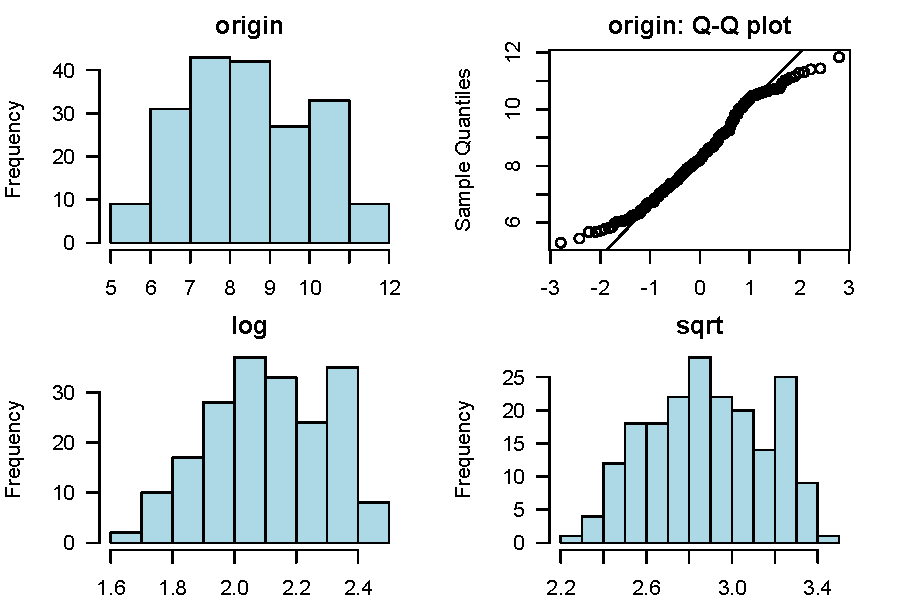
\includegraphics[width=1.0\textwidth]{figure/norm2.pdf}
\caption{logGDPpc2000}
\end{figure}
\clearpage
\subsubsection{ logGDPpc2015 }

normality test : Shapiro-Wilk normality test

\noindent statistic : 0.98126,  p-value : 0.0089949\\
\\% latex table generated in R 4.0.3 by xtable 1.8-4 package
% Tue Nov 10 19:09:30 2020
\begin{tabular}{lrr}
  \toprule
type & skewness & kurtosis \\ 
  \midrule
original & -0.0268 & 2.1397 \\ 
  log transformation & -0.3263 & 2.2943 \\ 
  sqrt transformation & -0.1746 & 2.1871 \\ 
   \bottomrule
\end{tabular}
\\
\begin{figure}[!ht]
\centering
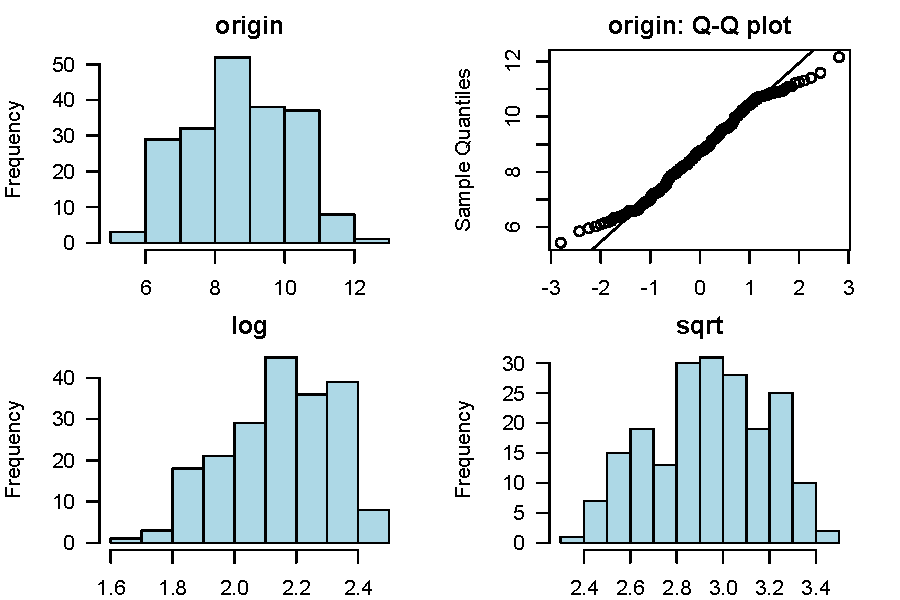
\includegraphics[width=1.0\textwidth]{figure/norm3.pdf}
\caption{logGDPpc2015}
\end{figure}
\clearpage
\subsubsection{ growthGDPpc }

normality test : Shapiro-Wilk normality test

\noindent statistic : 0.98337,  p-value : 0.0225057\\
\\% latex table generated in R 4.0.3 by xtable 1.8-4 package
% Tue Nov 10 19:09:30 2020
\begin{tabular}{lrr}
  \toprule
type & skewness & kurtosis \\ 
  \midrule
original & 0.4715 & 3.4139 \\ 
  log transformation & -1.4207 & 6.0170 \\ 
  sqrt transformation & 0.0311 & 2.5905 \\ 
   \bottomrule
\end{tabular}
\\
\begin{figure}[!ht]
\centering
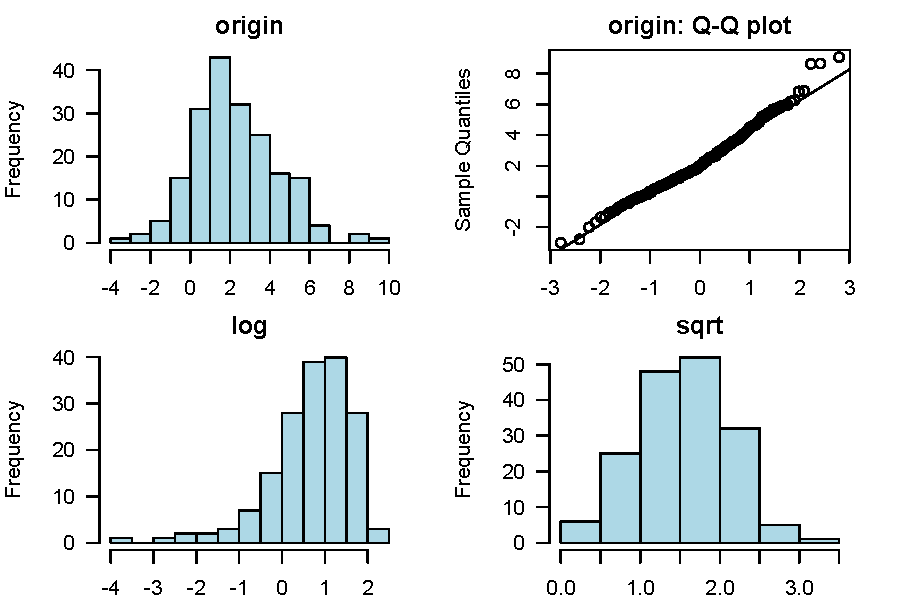
\includegraphics[width=1.0\textwidth]{figure/norm4.pdf}
\caption{growthGDPpc}
\end{figure}
\clearpage
\subsubsection{ imalaria2000 }

normality test : Shapiro-Wilk normality test

\noindent statistic : 0.80376,  p-value : 3.71679E-10\\
\\% latex table generated in R 4.0.3 by xtable 1.8-4 package
% Tue Nov 10 19:09:30 2020
\begin{tabular}{lrr}
  \toprule
type & skewness & kurtosis \\ 
  \midrule
original & 1.0566 & 3.1271 \\ 
  log transformation & -0.7556 & 3.3193 \\ 
  sqrt transformation & 0.4679 & 1.7609 \\ 
   \bottomrule
\end{tabular}
\\
\begin{figure}[!ht]
\centering
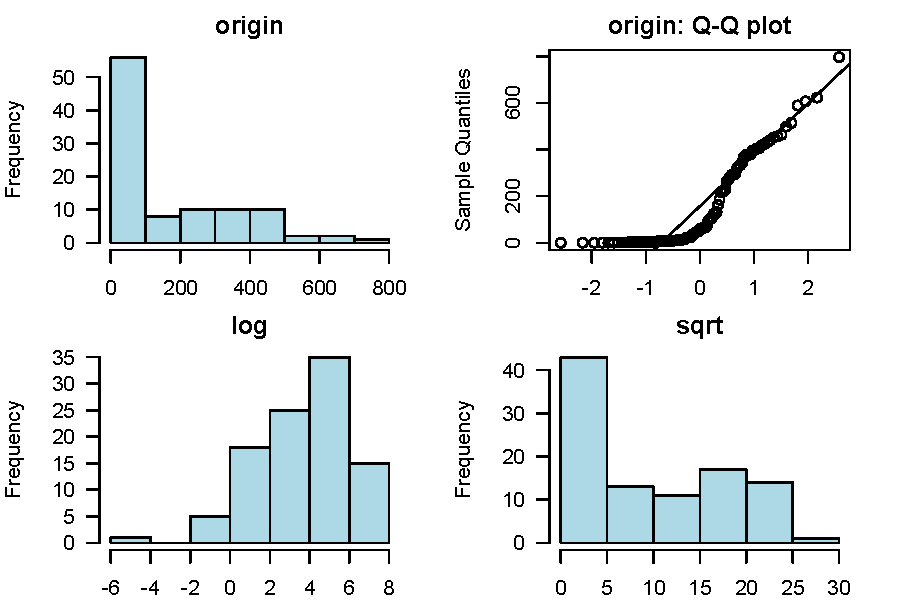
\includegraphics[width=1.0\textwidth]{figure/norm5.pdf}
\caption{imalaria2000}
\end{figure}
\clearpage
\subsubsection{ imalaria2015 }

normality test : Shapiro-Wilk normality test

\noindent statistic : 0.71267,  p-value : 1.26255E-12\\
\\% latex table generated in R 4.0.3 by xtable 1.8-4 package
% Tue Nov 10 19:09:30 2020
\begin{tabular}{lrr}
  \toprule
type & skewness & kurtosis \\ 
  \midrule
original & 1.2888 & 3.2152 \\ 
  log transformation &  &  \\ 
  sqrt transformation & 0.7632 & 2.0458 \\ 
   \bottomrule
\end{tabular}
\\
\begin{figure}[!ht]
\centering
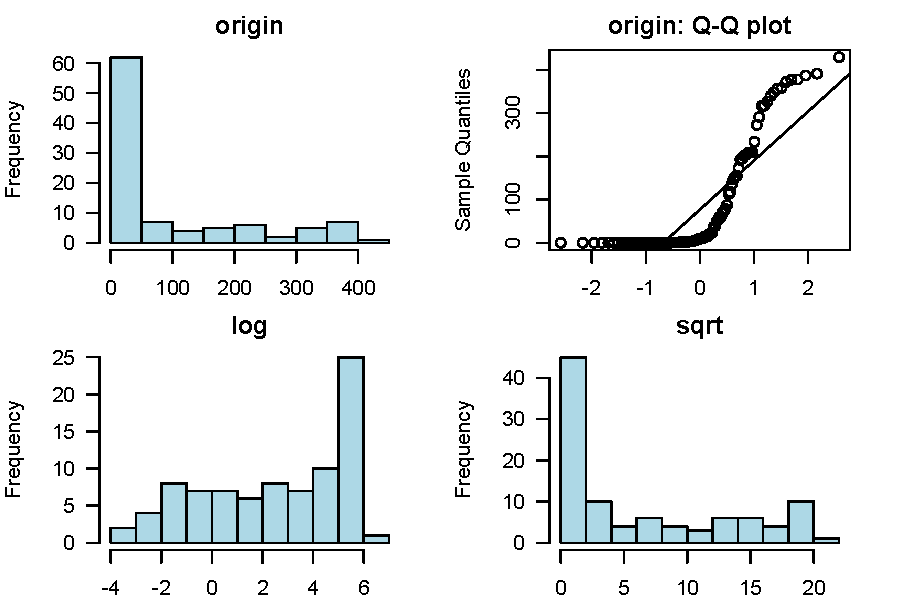
\includegraphics[width=1.0\textwidth]{figure/norm6.pdf}
\caption{imalaria2015}
\end{figure}
\clearpage
\subsubsection{ change\_malar }

normality test : Shapiro-Wilk normality test

\noindent statistic : 0.67302,  p-value : 1.56668E-13\\
\\% latex table generated in R 4.0.3 by xtable 1.8-4 package
% Tue Nov 10 19:09:30 2020
\begin{tabular}{lrr}
  \toprule
type & skewness & kurtosis \\ 
  \midrule
original & -2.9067 & 14.1567 \\ 
  log transformation & 0.0853 & 1.6011 \\ 
  sqrt transformation & 0.6666 & 2.2084 \\ 
   \bottomrule
\end{tabular}
\\
\begin{figure}[!ht]
\centering
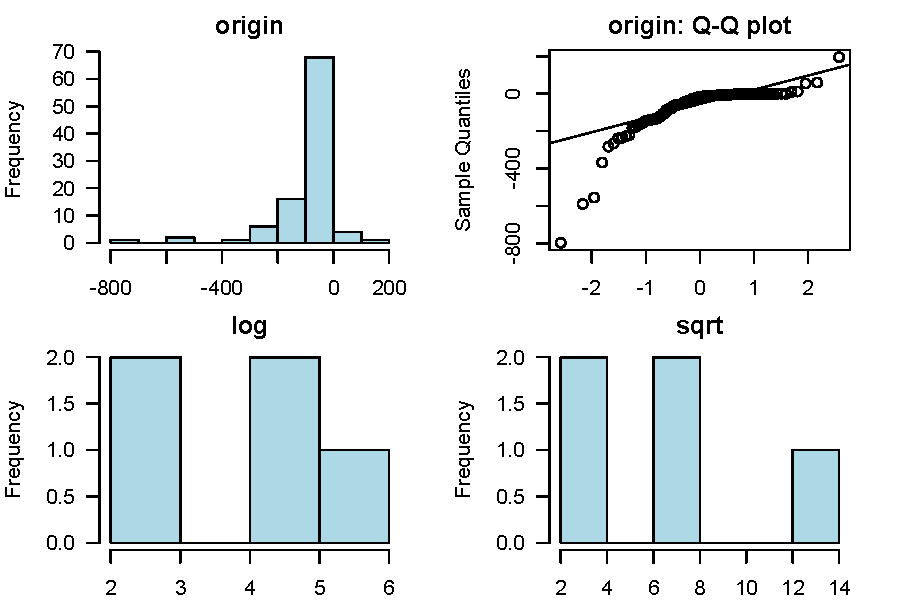
\includegraphics[width=1.0\textwidth]{figure/norm7.pdf}
\caption{change\_malar}
\end{figure}
\clearpage
\subsubsection{ educ\_sec }

normality test : Shapiro-Wilk normality test

\noindent statistic : 0.95245,  p-value : 0.00129114\\
\\% latex table generated in R 4.0.3 by xtable 1.8-4 package
% Tue Nov 10 19:09:30 2020
\begin{tabular}{lrr}
  \toprule
type & skewness & kurtosis \\ 
  \midrule
original & -0.2543 & 2.0154 \\ 
  log transformation & -1.4991 & 5.3899 \\ 
  sqrt transformation & -0.7400 & 2.9183 \\ 
   \bottomrule
\end{tabular}
\\
\begin{figure}[!ht]
\centering
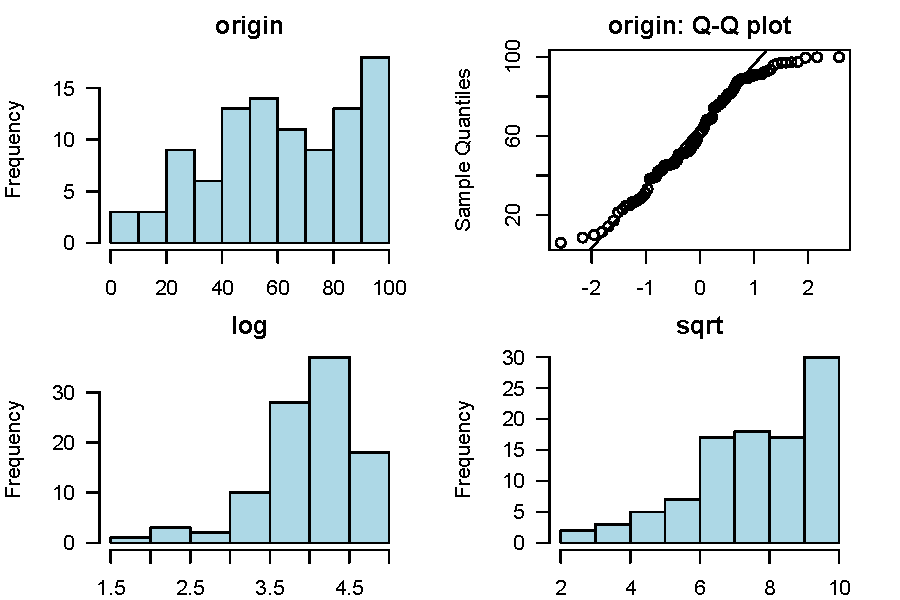
\includegraphics[width=1.0\textwidth]{figure/norm8.pdf}
\caption{educ\_sec}
\end{figure}
\clearpage
\subsubsection{ life2000 }

normality test : Shapiro-Wilk normality test

\noindent statistic : 0.91018,  p-value : 1.0976E-09\\
\\% latex table generated in R 4.0.3 by xtable 1.8-4 package
% Tue Nov 10 19:09:30 2020
\begin{tabular}{lrr}
  \toprule
type & skewness & kurtosis \\ 
  \midrule
original & -0.7728 & 2.4996 \\ 
  log transformation & -1.0014 & 2.9791 \\ 
  sqrt transformation & -0.8848 & 2.7134 \\ 
   \bottomrule
\end{tabular}
\\
\begin{figure}[!ht]
\centering
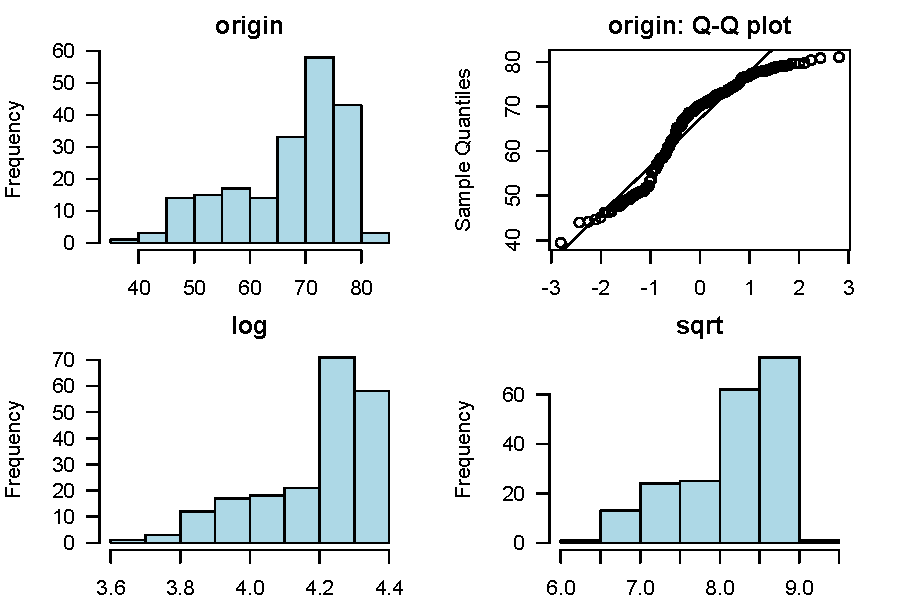
\includegraphics[width=1.0\textwidth]{figure/norm9.pdf}
\caption{life2000}
\end{figure}
\clearpage
\subsubsection{ trade2000 }

normality test : Shapiro-Wilk normality test

\noindent statistic : 0.85759,  p-value : 6.95547E-12\\
\\% latex table generated in R 4.0.3 by xtable 1.8-4 package
% Tue Nov 10 19:09:30 2020
\begin{tabular}{lrr}
  \toprule
type & skewness & kurtosis \\ 
  \midrule
original & 1.9988 & 9.9260 \\ 
  log transformation & -1.6383 & 12.9331 \\ 
  sqrt transformation & 0.6646 & 4.8121 \\ 
   \bottomrule
\end{tabular}
\\
\begin{figure}[!ht]
\centering
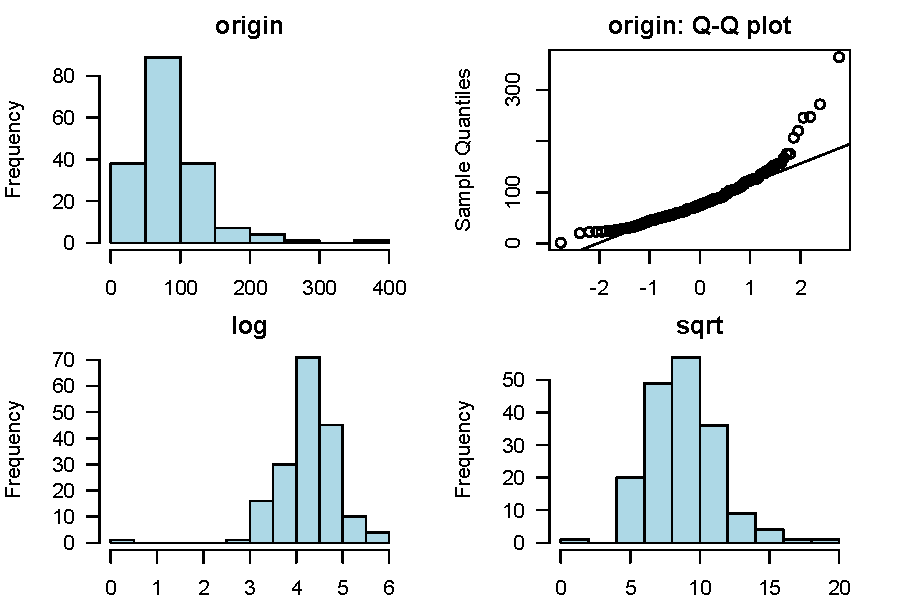
\includegraphics[width=1.0\textwidth]{figure/norm10.pdf}
\caption{trade2000}
\end{figure}
\clearpage
\subsubsection{ gov2000 }

normality test : Shapiro-Wilk normality test

\noindent statistic : 0.9637,  p-value : 6.99535E-05\\
\\% latex table generated in R 4.0.3 by xtable 1.8-4 package
% Tue Nov 10 19:09:30 2020
\begin{tabular}{lrr}
  \toprule
type & skewness & kurtosis \\ 
  \midrule
original & 0.4311 & 2.5550 \\ 
  log transformation & -1.6500 & 6.3651 \\ 
  sqrt transformation & -0.2052 & 2.0131 \\ 
   \bottomrule
\end{tabular}
\\
\begin{figure}[!ht]
\centering
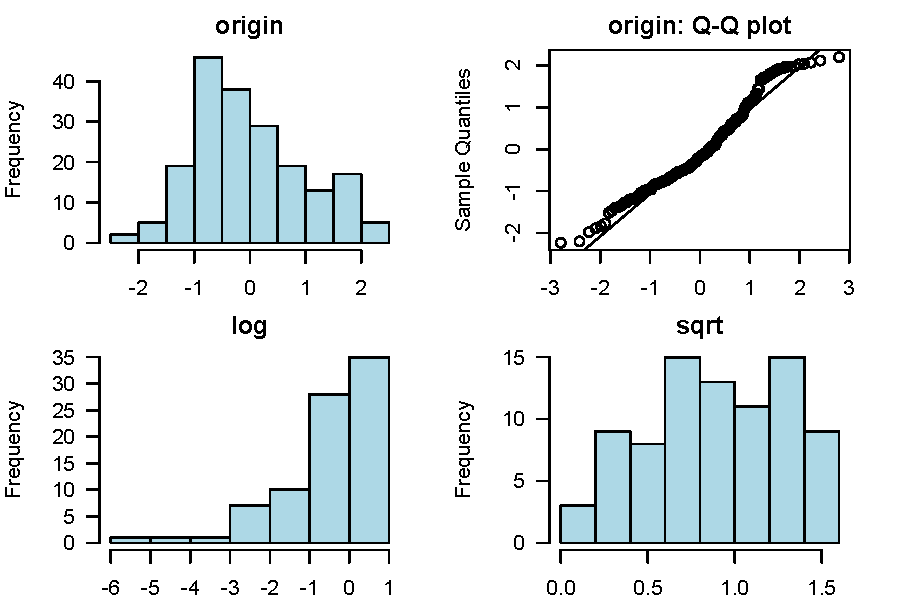
\includegraphics[width=1.0\textwidth]{figure/norm11.pdf}
\caption{gov2000}
\end{figure}
\clearpage
\subsubsection{ invest\_growth }

normality test : Shapiro-Wilk normality test

\noindent statistic : 0.95295,  p-value : 0.000231148\\
\\% latex table generated in R 4.0.3 by xtable 1.8-4 package
% Tue Nov 10 19:09:30 2020
\begin{tabular}{lrr}
  \toprule
type & skewness & kurtosis \\ 
  \midrule
original & 1.0003 & 5.8176 \\ 
  log transformation & -1.2261 & 5.6779 \\ 
  sqrt transformation & 0.2515 & 3.2722 \\ 
   \bottomrule
\end{tabular}
\\
\begin{figure}[!ht]
\centering
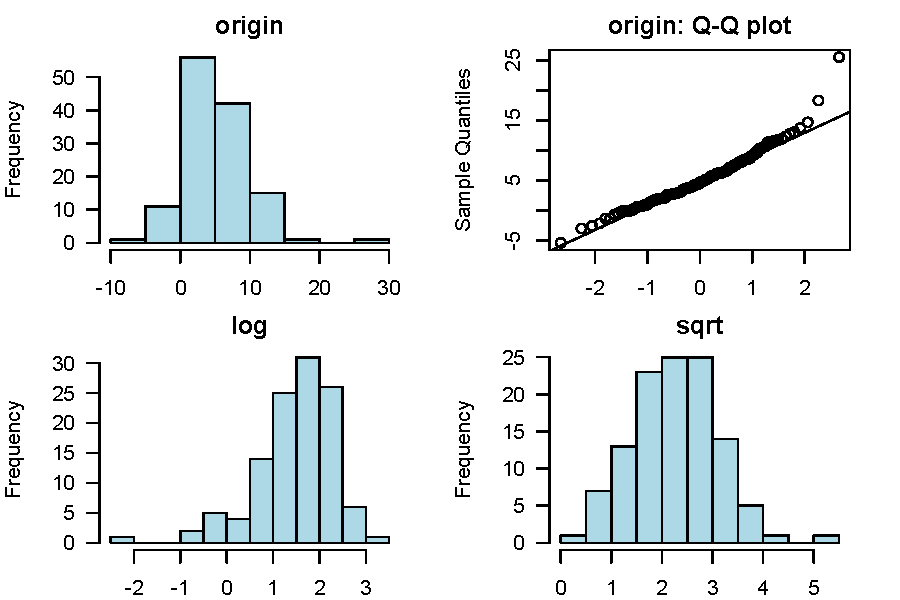
\includegraphics[width=1.0\textwidth]{figure/norm12.pdf}
\caption{invest\_growth}
\end{figure}
\clearpage

\chapter{Relationship Between Variables}
\section{Correlation Coefficient}
\subsection{Correlation Coefficient by Variable Combination}

\begin{longtable}[t]{llr}
\caption{\label{tab:correlations}The correlation coefficients (0.5 or more)}\\
\toprule
Variable1 & Variable2 & Correlation Coefficient\\
\midrule
\endfirsthead
\caption[]{The correlation coefficients (0.5 or more) \textit{(continued)}}\\
\toprule
Variable1 & Variable2 & Correlation Coefficient\\
\midrule
\endhead

\endfoot
\bottomrule
\endlastfoot
\cellcolor{gray!6}{logGDPpc2015} & \cellcolor{gray!6}{logGDPpc2000} & \cellcolor{gray!6}{0.980}\\
gov2000 & logGDPpc2000 & 0.815\\
\cellcolor{gray!6}{life2000} & \cellcolor{gray!6}{logGDPpc2015} & \cellcolor{gray!6}{0.812}\\
gov2000 & logGDPpc2015 & 0.808\\
\cellcolor{gray!6}{life2000} & \cellcolor{gray!6}{logGDPpc2000} & \cellcolor{gray!6}{0.790}\\
\addlinespace
change\_malar & imalaria2000 & -0.743\\
\cellcolor{gray!6}{imalaria2015} & \cellcolor{gray!6}{imalaria2000} & \cellcolor{gray!6}{0.726}\\
life2000 & imalaria2015 & -0.702\\
\cellcolor{gray!6}{gov2000} & \cellcolor{gray!6}{life2000} & \cellcolor{gray!6}{0.673}\\
invest\_growth & logGDPpc2000 & -0.566\\
\addlinespace
\cellcolor{gray!6}{life2000} & \cellcolor{gray!6}{imalaria2000} & \cellcolor{gray!6}{-0.566}\\
invest\_growth & life2000 & -0.541\\
\cellcolor{gray!6}{imalaria2015} & \cellcolor{gray!6}{logGDPpc2015} & \cellcolor{gray!6}{-0.532}\\
invest\_growth & logGDPpc2015 & -0.514\\
\cellcolor{gray!6}{educ\_sec} & \cellcolor{gray!6}{imalaria2015} & \cellcolor{gray!6}{-0.514}\\
\addlinespace
invest\_growth & imalaria2015 & 0.503\\*
\end{longtable}

\subsection{Correlation Plot of Numerical Variables}
\begin{figure}[!ht]
\centering
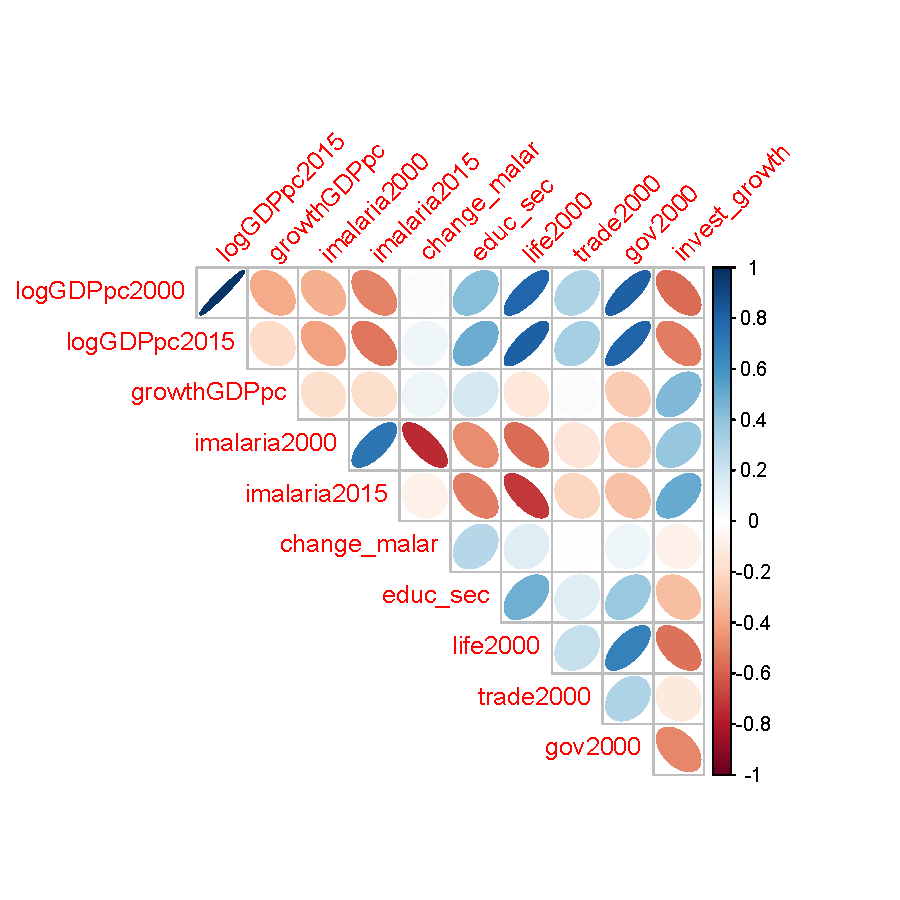
\includegraphics[width=0.99\textwidth]{figure/correlation.pdf}
\caption{The correlation coefficient of numerical variables}
\end{figure}


\chapter{Target based Analysis}
\section{Grouped Descriptive Statistics}
\subsection{Grouped Numerical Variables}

There is no target variable.



\subsection{Grouped Categorical Variables}

There is no target variable.



\section{Grouped Relationship Between Variables}
\subsection{Grouped Correlation Coefficient}
There is no target variable.



\subsection{Grouped Correlation Plot of Numerical Variables}
There is no target variable.






\end{document}
